% TODO
% . include figures

\section{Faster Candidate Motif Elimination through Block Processing}

The EMS-GT algorithm tests candidate motifs in a brute-force approach. A candidate motif is tested by checking if it has at least one $d$-neighbor in each of the remaining $n - n'$ sequences. In testing a candidate motif $c$, if there is a sequence $S_i$ in the remaining $n - n'$ sequences where $c$ doesn't have any $d$-neighbor, candidate motif $c$ is automatically eliminated.

In our implementation, the search space is represented by a compressed bit array and the $l$-mers are enumerated alphabetically. $L$-mers that are near each other do not differ that much. We used this observation in improving the way the algorithm tests the candidate motifs. Figure 1 illustrates a part of the search space's representation.

% include search space, 
\begin{figure}[h]
	\centering
	\label{fig:search_space}
	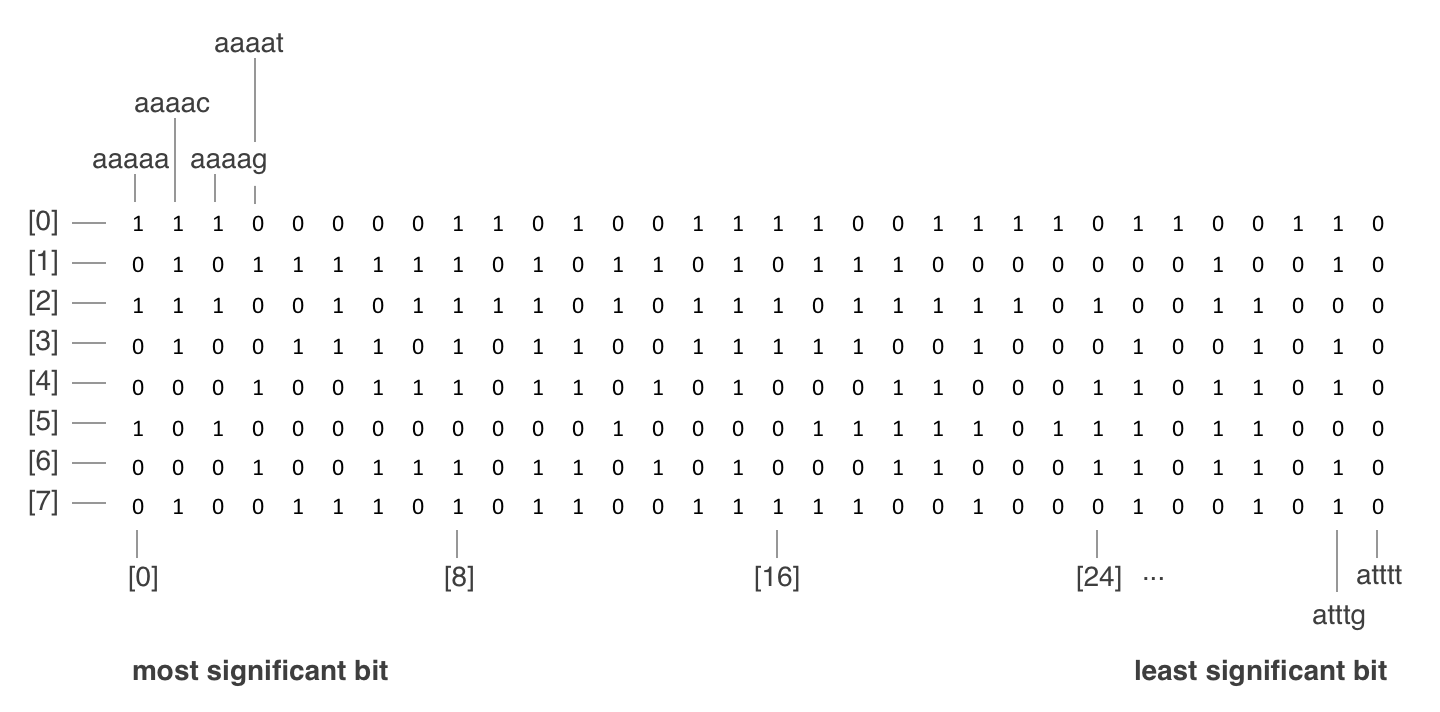
\includegraphics[width=5in]{contents/00_images/search_space}\vspace*{5pt}
	\caption{First 8 rows of the $4^{5}$ search space with random flag values.}
\end{figure}

In EMS-GT, each testing of candidate motif is independent of each other. We proposed a speedup technique that processes these candidate motifs by blocks. We first partition the search space by blocks containing $4^k$ $l$-mers. This results into $l$-mers that share the same $(l-k)$-prefix characters where $2 < k < l$. Since every row in the search space represents exactly 32 $l$-mers (32-bit integers), the height of every block is computed using $(4^k / 32)$. Additionally, any two $l$-mers within a block has at most $k$ hamming distance value between them. Figure 2 shows an example of partitioned search space showing blocks of $l$-mers sharing a common prefix string. In our implementation we use $k = 5$ and every block has a height of 32.

% include figure that shows how we partition the search space
\begin{figure}[h]
	\centering
	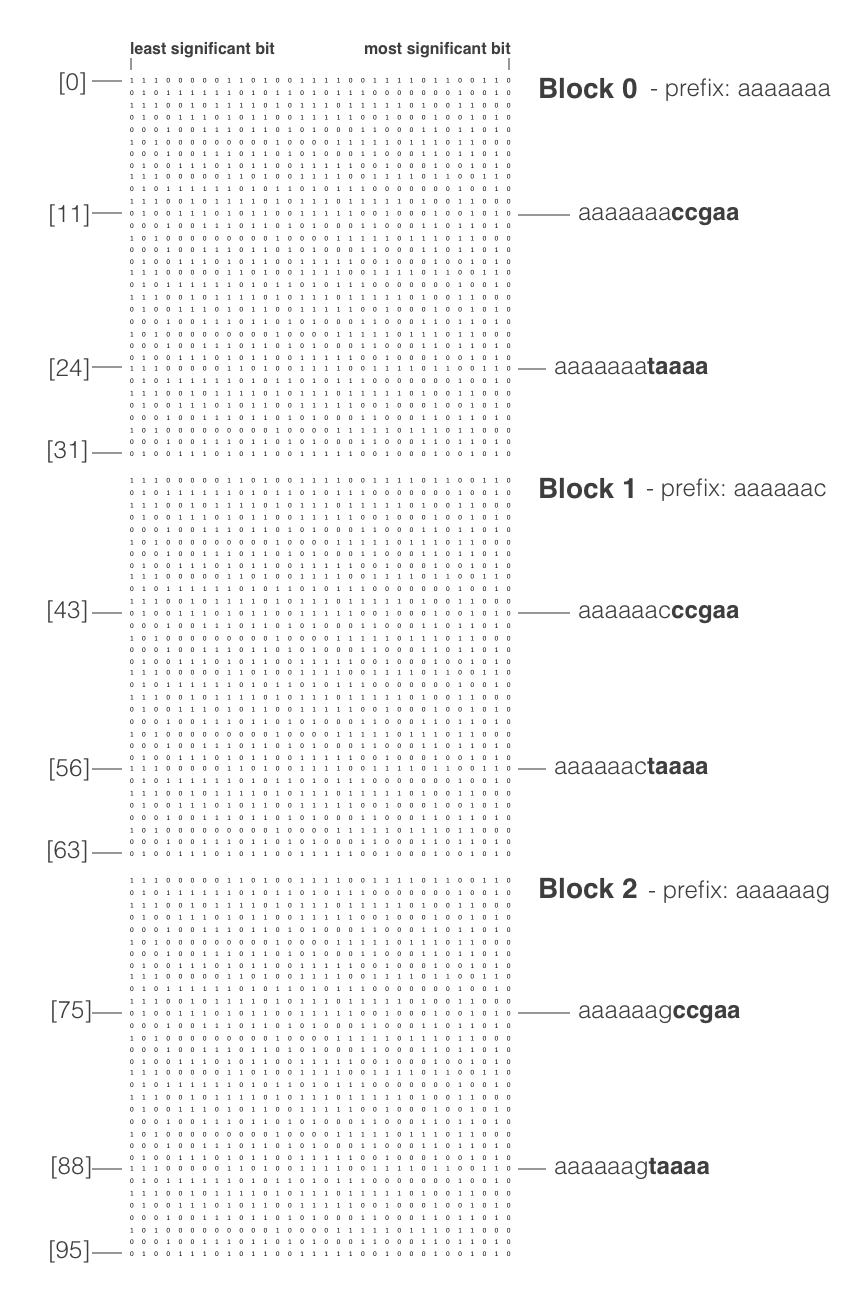
\includegraphics[width=3.0in]{contents/00_images/block_search_space}\vspace*{5pt}
	
	\caption{Illustration of the block partitioning of a $4^{12}$ search space. There are $4^{5}$ $l$-mers in each block and has a height of 32. The illustration shows the first 3 blocks only.}
	\label{fig:block_search_space}
\end{figure}

We process the testing of candidate motifs now by blocks. If candidate motifs $x$ and $y$ are within a block and $x$ has been eliminated as a candidate motif in sequence $S_i$ $(n' \leq i \leq n)$, we can filter out $l$-mers $z \in S_i$ where $d_H(x,z) > d + k$. We collect the remaining $l$-mers in $S_i$ and use it for testing the remaining candidate motifs in the block along with the other $l$-mers in the remaining sequences in ${S_n', S_n'+1, ..., S_n} - {S_i}$. The theorem below formalizes the main property used in this speedup technique.

\begin{thm} \label{thm:triangle}
	Let x and y be $l$-mers in a block in the search space containing $4^k$ $l$-mers. Let $d$ be the number of allowed mutations in the problem instacne. Let z be another $l$-mer. If $d_H(x, z) > (k + d)$ then $d_H(y, z) > d$ and therefore $z$ is not in $N(y, d)$
\end{thm}

\begin{proof}[Proof of Theorem \ref{thm:triangle}]
Using proof by contradiction, we first suppose that $d_H(y, z) \leq d$. Since the $l$-mers $x$ and $y$ belong to the same block, then $d_H(x, y) \leq k$. We use these bound in the triangle of inequality $d_H(x, z) \leq d_H(x, y) + d_H(y, z)$ to derive the result $d_H(x, z) \leq k + d$ . This result contradicts the given condition that $d_H(x, z) > (k + d)$. Hence, we are sure that $d_H(y, z) > d$.
\end{proof}

The $k$-value affects the number of $l$-mers that is filtered in a sequence. The lower its value, the larger the number of filtered $l$-mers and faster candidate motif testing will be. But since $k$ also affects the number of $l$-mers in a block, the lower its value, the fewer the candidate motifs that might benefit from the speedup technique. In our implementation we use $k = 5$ where every block is 32 rows of 32 bit flags representing a total of $4^5$ $l$-mers.

